\documentclass[11pt]{article}
\usepackage[T1]{fontenc}
\usepackage{lmodern}
\usepackage{amsmath,amssymb,amsthm}
\usepackage[margin=1.1in]{geometry}
\usepackage{microtype}
\usepackage{tikz}
\usetikzlibrary{arrows.meta}
\usepackage[hidelinks]{hyperref}
\newtheorem{theorem}{Theorem}[section]
\newtheorem{proposition}[theorem]{Proposition}
\newtheorem{lemma}[theorem]{Lemma}
\newtheorem{corollary}[theorem]{Corollary}
\theoremstyle{remark}
\newtheorem{remark}[theorem]{Remark}
\pdfinfoomitdate=1
\pdftrailerid{}
\pdfsuppressptexinfo=15
\title{A group without fixed price}
\author{OpenAI}
\date{October 5, 2026}
\begin{document}
\maketitle
\begin{abstract}
We construct a finitely generated group with two essentially free
probability-measure-preserving actions of different costs. This gives
a negative answer to Gaboriau's general fixed-price problem. The group is an
amalgam of a free group of rank $100$ with a direct product. Its
Bernoulli action has cost bounded away from one, whereas finite height
extensions have costs tending to one.
\end{abstract}
\tableofcontents
\section{Introduction}

The cost of an action measures how many edges, on average, are needed
to connect its orbits. More precisely, let a countable group $\Gamma$
act by measure-preserving Borel automorphisms on a standard probability
space $(X,\mu)$. We use right actions, so $(xg)h=x(gh)$.
Its orbit relation is
\[
 \mathcal R=\{(x,xg):x\in X,\ g\in\Gamma\}.
\]
A \emph{graphing} $\mathcal E$ of $\mathcal R$ is a countable family of
measure-preserving Borel bijections between Borel subsets of $X$,
with graphs contained in $\mathcal R$. It generates $\mathcal R$ if
finite paths in these maps and their inverses connect all related
points on a conull set. Its cost $C(\mathcal E)$ is the sum of its domain measures;
$\operatorname{Cost}(\mathcal R)$ is the infimum of these sums over
generating graphings. An action is \emph{essentially free} if each
nonidentity group element fixes a null set. A group has \emph{fixed
price} if all its essentially free probability-measure-preserving
(p.m.p.) actions have the same cost.

Levitt introduced cost \cite{levitt-1995}. Gaboriau developed its
connections with group theory and the fixed-price problem
\cite{gaboriau-2000}. His work shows, in particular, that free groups
have fixed price equal to their rank, and establishes fixed price one
for many groups with commuting or amenable structure. Recent results
include the fixed-price-one theorem for products of two infinite
countable groups \cite{khezeli-2026-v4}, metric and infinite-measure
action criteria \cite{bevilacqua-bowen-2025-v1}, and a criterion based
on small product neighborhoods of finite subsets
\cite{slutsky-2026-v1}. We give a group for which fixed price fails.

\subsection{The group and the two actions}

Let
\[
 A=F(a,b_1,\ldots,b_{99}),\qquad
 w=ab_1ab_2\cdots ab_{99}a,
 \qquad J=\langle b_1,\ldots,b_{99},w\rangle\le A.
\]
Let $\langle t\rangle$ be infinite cyclic and set
\begin{equation}\label{intro:group}
 \Gamma=A*_J(J\times\langle t\rangle).
\end{equation}
The homomorphism $\chi:\Gamma\to\mathbb Z$ given by
$\chi(a)=1$ and $\chi(b_i)=\chi(t)=0$ is well defined; note that
$\chi(w)=100$. On the Bernoulli
probability space $X_0=[0,1]^\Gamma$ with product Lebesgue measure, let
\[
 (xg)(h)=x(gh).
\]
Let $X\subseteq X_0$ be the invariant conull set of points with trivial
stabilizer, equipped with the restricted probability measure. For an
integer $M>100$, give $Y_M=X\times\mathbb Z/M\mathbb Z$
product measure with uniform height coordinate, and define
\[
 (x,r)g=(xg,r+\chi(g)\bmod M).
\]
Both actions are free; restriction from $X_0$ to $X$ preserves cost.
Their elementary group-theoretic
and measure-theoretic properties are proved in Section~\ref{actions:section}.

\begin{theorem}\label{intro:main}
Put $K=e^{96}96^{99}/95^{95}$, choose
\[
 0<\alpha<1/200,\qquad K\alpha^3<1/2,
 \qquad \eta=\alpha/100.
\]
For the group and actions just defined,
\[
 \operatorname{Cost}(\mathcal R_{\Gamma\curvearrowright X})
      \ge1+\eta,
 \qquad
 \operatorname{Cost}(\mathcal R_{\Gamma\curvearrowright Y_M})
      \le1+\frac{99}{M}\quad(M>100).
\]
In particular, choosing an integer $M>\max\{100,99/\eta\}$ gives
two essentially free p.m.p. actions of the same finitely generated
group with strictly different costs. Thus the general fixed-price
assertion is false.
\end{theorem}

\subsection{How the proof works}

The upper bound uses the finite height coordinate. All $t$-edges,
together with the generators of $J$ on a small set meeting every
$t$-orbit, generate the $J\times\langle t\rangle$ relation at cost
arbitrarily close to one. It remains to add $a$-edges. The relation
$w=ab_1\cdots ab_{99}a$ propagates $a$-edges from any $99$
consecutive heights to the next height, so an initial cost $99/M$
is enough.

For the lower bound, write $\mathcal R_A$ and $\mathcal R_J$ for
the restricted orbit relations on $X$, and define the relative
quantity
\[
 \delta_X=\inf\{C(\mathcal E):
       \mathcal R_J\vee\mathcal E=\mathcal R_A,
       \ \mathcal E\subseteq\mathcal R_A\}.
\]
Here $C(\mathcal E)$ is the graphing cost, and the join denotes the
relation generated by the supplied $\mathcal R_J$-steps and the
edges of $\mathcal E$. Three steps give the desired bound:
\begin{enumerate}
\item \emph{Deploy and compress graphings.}
Subdivide a nearly optimal $\Gamma$-graphing into factor edges on a
larger finite-measure space. Repeated compression makes more of the
$J$-relation available and recovers its exact saved cost. Amalgam
normal form then gives
$\operatorname{Cost}(\mathcal R_\Gamma)\ge1+\delta_X$.
The construction follows Gaboriau's deployment method
\cite[\S\,IV.28--IV.32 and Proposition~IV.35]{gaboriau-2000};
Sections~\ref{compression:section}--\ref{deployment:section}
prove the required relative estimate directly.
\item \emph{Pass to finite permutation models.}
Put $u_0=1$ and $u_i=u_{i-1}ab_i$ for $1\le i\le99$. A finite set $V$ with a right
$A$-action by permutations defines a group whose symbols record
$a$-steps, while all $J$-steps are assigned the identity:
\[
 D_V=\langle x_v\ (v\in V)\mid
              x_vx_{vu_1}\cdots x_{vu_{99}}=1\ (v\in V)\rangle.
\]
Write $\operatorname{rk}(D_V)$ for its minimum number of generators.
Local approximation of Bernoulli graphings gives
$\delta_X\ge\limsup\operatorname{rk}(D_V)/|V|$ along any
asymptotically free sequence of such models, meaning that each fixed
nonidentity element of $A$ fixes a fraction of points tending to zero.
The displayed row makes $w$ trivial in this encoding. In
Section~\ref{models:section}, random permutations supply models with
strong expansion and few overlapping relators.
\item \emph{Bound the rank by shortening a labelled graph.}
The expansion property forces
$\operatorname{rk}(D_V)>\eta|V|$ for large models. A minimal
labelled graph representing a generating set would otherwise contain
a long relator segment that could be replaced by a shorter path.
This uses the Arzhantseva--Ol'shanskii method
\cite{arzhantseva-olshanskii-1996,kapovich-schupp-2002}.
The additional ingredients are a saturation procedure for exceptional
letters and a planar word lemma over an arbitrary coefficient group,
proved in Sections~\ref{planar:section} and~\ref{rank:section}.
\end{enumerate}

The proof isolates three estimates beyond this example: compression
relative to a supplied equivalence relation, a transfer from Bernoulli
graphings to ranks of finitely presented groups, and a deterministic
rank bound from expansion with sparse overlaps. Their statements
specify their own inputs and conclusions. The coefficient group is the actual subgroup generated by the letters
absorbed during saturation. It need not be finitely presented: all
relations true in that subgroup are retained, so its injection into the
presented group is part of the construction. The planar lemma keeps
track of these coefficient values while counting only the remaining
letters.

\section{The group and an action of small cost}
\label{actions:section}

We construct the group and two free probability-measure-preserving actions
that will be compared.  The purpose of this section is to prove the upper
bound for the action with an additional finite height coordinate.
All actions are right actions: $(zg)h=z(gh)$.

\subsection{The amalgam}

Let $A=F(a,b_1,\ldots,b_{99})$ be the free group on the
displayed generators.  Define words in $A$ by
\[
 u_0=1,\qquad u_i=u_{i-1}ab_i\quad(1\leq i\leq99),
 \qquad w=u_{99}a.
\]
Let
\begin{equation}
 \label{actions:group}
 J=\langle b_1,\ldots,b_{99},w\rangle\leq A,
 \qquad B=J\times\langle t\rangle,
 \qquad \Gamma=A*_J B,
\end{equation}
where $\langle t\rangle$ is infinite cyclic and the embedding of $J$ in
$B$ is $j\mapsto(j,1)$.

\begin{lemma}
\label{actions:normal-form}
The factors $A$ and $B$ embed in $\Gamma$ with intersection $J$.
If $g_1,\ldots,g_n$ lie alternately in $A\setminus J$ and
$B\setminus J$, then $g_1\cdots g_n\notin J$ for $n\geq1$, and
$g_1\cdots g_n$ belongs to neither factor for $n\geq2$.
The group $J$ is free on $b_1,\ldots,b_{99},w$; in particular it is
infinite.  The group $\Gamma$ is countably infinite and generated by
$a,b_1,\ldots,b_{99},t$.
\end{lemma}

\begin{proof}
Choose, in each factor, representatives for the cosets $gJ$, with $1$
representing $J$.  Consider formal strings
\[
 r_1\cdots r_n j,
 \qquad j\in J,
\]
where the $r_i$ are nonidentity representatives, alternately from the
two factors; the case $n=0$ is allowed.  Define right multiplication by
$g$ in one factor as follows.  If the last representative is from that
factor, combine it with the final $j$ and $g$, and write their product
uniquely as $rj'$ in that factor.  Otherwise write $jg=rj'$ and append
$r$.  Omit $r$ when $r=1$.

This gives a right action of each factor on the strings.  To check the
action law for two successive multipliers in the same factor, retain
the prefix ending in the other factor and simply multiply the remaining
suffix in the chosen factor.  This description continues to apply when
the suffix representative becomes $1$.  The two actions agree for
multipliers in $J$, which only multiply the final $J$-entry.  They
therefore define an action of the amalgam on the strings.

Acting on the identity string by a factor element recovers its coset
decomposition, so the factors embed.  Their possible strings intersect
exactly in the strings with no representatives, proving $A\cap B=J$.
Successively multiplying by an alternating sequence outside $J$
adds one nonidentity representative at every step: for $j\in J$ and
$g\notin J$, one has $jg\notin J$.  The resulting string has length
$n$, whereas elements of $J$ have length zero and factor elements have
length at most one.  This proves the stated normal-form assertions.

For $J$, expand any reduced nonempty word in the abstract generators
$b_1,\ldots,b_{99},w$ in the free basis of $A$.
The word $w=ab_1ab_2\cdots ab_{99}a$ starts and ends with $a$;
$w^{-1}$ starts and ends with $a^{-1}$.  No boundary between a
$b_i^{\pm1}$ and $w^{\pm1}$ cancels.  Two successive $w$-symbols
either have equal signs, in which case their boundary does not cancel,
or would be inverse symbols, which reducedness excludes.  Boundaries
between $b$-symbols do not cancel either.  Thus the expansion is a
nonempty reduced word in $A$, proving that the displayed generators of
$J$ are a free basis.

Finally, the displayed generators of $\Gamma$ generate both factors;
the embedded copy of $A$ makes $\Gamma$ infinite, and finite generation
makes it countable.  The embedded copy of $B$ also shows that $t$ has
infinite order in $\Gamma$.
\end{proof}

\subsection{Probability spaces and the two actions}

We use the definitions of graphing, cost, and p.m.p. action from the
introduction. A standard Borel space is a measurable space isomorphic
to a Borel subset of a complete separable metric space. For a subgroup
$L\leq\Gamma$, write $\mathcal R_L$ for its orbit relation on the
space being considered.

For an essentially free action of a countable group, the set of points with trivial stabilizer is a Borel invariant
conull set.  Restricting
to this set makes the action pointwise free and preserves the measure
and orbit-relation cost.  More generally, a Borel conull set can be
made invariant by intersecting its countably many translates.
To see that an invariant conull restriction preserves cost, restrict
any orbit graphing to that set; invariance keeps its edges inside
the set, and domain measures do not change.  Conversely, a graphing
on the restricted set generates the original relation on a conull
set and has the same cost when viewed on the original space.

Let
\[
 X_0=[0,1]^\Gamma,\qquad
 \mu_0=\operatorname{Leb}^{\Gamma},\qquad
 (xg)(h)=x(gh)\quad(g,h\in\Gamma).
\]
This is a standard Borel probability space, since it is a countable
product of compact metrizable spaces, with its product measure.
Coordinate permutations are Borel automorphisms preserving $\mu_0$,
and the displayed formula satisfies the right-action law.  For
$g\ne1$, the equality $xg=x$ implies $x(g)=x(1)$.  These are two
independent uniform coordinates, so this equality has probability zero.
Consequently
\[
 X=\{x\in X_0:xg\ne x\text{ for every }g\ne1\}
\]
is an invariant Borel conull set.  Write $\mu$ for the restricted
probability measure.  We henceforth use the free Bernoulli action on
$(X,\mu)$; it has the same orbit-relation cost as the original action
on $(X_0,\mu_0)$.

\begin{lemma}
\label{actions:height}
There is a homomorphism $\chi:\Gamma\to\mathbb Z$ with
\[
 \chi(a)=1,\qquad \chi(b_i)=\chi(t)=0.
\]
It satisfies $\chi(u_i)=i$ and $\chi(w)=100$.
For every positive integer $M$, the action on
\[
 Y_M=X\times\mathbb Z/M\mathbb Z,
 \qquad \nu_M=\mu\times\text{uniform measure},
\]
defined by
\begin{equation}
 \label{actions:product-action}
 (x,r)g=(xg,r+\chi(g)\bmod M)
\end{equation}
is free and p.m.p. on a standard Borel probability space.
\end{lemma}

\begin{proof}
The exponent sum of $a$ defines a homomorphism $\chi_A:A\to\mathbb Z$.
Define $\chi_B(jt^n)=\chi_A(j)$ on $B=J\times\langle t\rangle$.
This is a homomorphism and agrees with $\chi_A$ on $J$, so the
amalgam's universal property gives $\chi$.  The formulas for $u_i$
and $w$ follow by their definitions.  In particular, the restriction
of $\chi$ to $J$ need not be zero: it sends $w$ to $100$.
The homomorphism law verifies the right-action law in
\eqref{actions:product-action}.  Both coordinate actions preserve
their measures.  Freeness follows from freeness on the first
coordinate, and the finite product remains standard Borel.
\end{proof}

\subsection{A graphing on the height extension}

The direct-product factor $B$ can be generated at arbitrarily small
cost above one by retaining all $t$-edges and using the generators of
$J$ on a small set meeting every $t$-orbit.  This is the product
construction in Gaboriau's Proposition~VI.23
\cite[Proposition~VI.23]{gaboriau-2000}.  For our Bernoulli action the
small set has the following explicit description.

\begin{lemma}
\label{actions:small-marker}
For every $0<p<1$ and every positive integer $M$, there is a Borel
set $C_p\subseteq Y_M$ of measure $p$ meeting every
$\langle t\rangle$-orbit.  The graphing consisting of $t$ on all
of $Y_M$ and $b_1,\ldots,b_{99},w$ restricted to $C_p$ generates
$\mathcal R_B$ and has cost $1+100p$.
\end{lemma}

\begin{proof}
In $X$, put
\[
 N_p=\{x\in X:x(t^n)\geq p\text{ for every }n\in\mathbb Z\},
 \qquad
 C_p=(\{x\in X:x(1)<p\}\cup N_p)\times\mathbb Z/M\mathbb Z.
\]
The set $N_p$ is Borel, invariant under $t$, and null: the coordinates
$x(t^n)$ are independent, and the group elements $t^n$ are distinct.
Indeed, the probability that the condition holds for $0\leq n<N$
is $(1-p)^N$.  Thus $\nu_M(C_p)=p$.
If a $t$-orbit does not meet the first part of $C_p$, all its points
belong to $N_p\times\mathbb Z/M\mathbb Z$.  Hence $C_p$ meets every
$t$-orbit, including the exceptional ones.

Let $j$ be one of $b_1,\ldots,b_{99},w$, and let $z\in Y_M$.
Choose $n\in\mathbb Z$ with $zt^n\in C_p$.  The graphing contains
the path
\[
 z\longrightarrow zt^n\longrightarrow zt^nj
   \longrightarrow zt^njt^{-n}=zj,
\]
where the first and last portions use $t$ or $t^{-1}$.  The final
identity uses $jt=tj$ in $B$.  Thus every generator of $B$ is
available everywhere in the generated relation.  Conversely, all
the graphing's maps are restrictions of elements of $B$.
Each of the $100$ restricted generators costs $p$, and the full
$t$-map costs one.
\end{proof}

\begin{proposition}
\label{actions:low}
For every integer $M>100$, the free p.m.p. action
$\Gamma\curvearrowright(Y_M,\nu_M)$ of
\eqref{actions:product-action} satisfies
\[
 \operatorname{Cost}(\mathcal R_{\Gamma\curvearrowright Y_M})
 \leq1+\frac{99}{M}.
\]
\end{proposition}

\begin{proof}
Fix $0<p<1$ and use the graphing of
Lemma~\ref{actions:small-marker}.  Add the restriction of $a$ to
the union of the height fibers $0,1,\ldots,98$.  Its domain has
measure $99/M$, so the resulting graphing has cost
\[
 1+100p+\frac{99}{M}.
\]
Let $E$ be the equivalence relation it generates.  It contains
$\mathcal R_B$, and we will prove that it contains every $a$-edge.

Suppose that $(z,za)\in E$ whenever the height of $z$ is one of
$k,k+1,\ldots,k+98$, interpreted modulo $M$.  Given $z$ at height
$k+99$, set $y=zu_{99}^{-1}$, which has height $k$.
The sequence
\[
 y=yu_0,\quad yu_1,\quad\ldots,\quad yu_{99}=z
\]
is connected by $E$: at its $i$th step apply $a$ to $yu_{i-1}$,
of height $k+i-1$, and then apply $b_i$.  The $a$-edge is among
those assumed available, and the $b_i$-edge belongs to
$\mathcal R_B$.  The $w$-edge also belongs to $\mathcal R_B$, and
\[
 yw=yu_{99}a=za.
\]
Thus $z$ and $za$ are $E$-equivalent, proving the implication from
$99$ consecutive known source heights to the next one.

The heights $0,\ldots,98$ are known initially.  Apply this
implication for the ordinary integers
$k=0,1,\ldots,M-100$.  It successively supplies source heights
$99,100,\ldots,M-1$; the last $a$-edges end at height $0$ modulo
$M$, as required.  Hence all $a$-edges lie in $E$.
Since $B$ and $a$ generate $\Gamma$, this graphing generates
$\mathcal R_\Gamma$.  Taking the infimum over graphings and then
letting $p\downarrow0$ proves the bound.
\end{proof}

\section{Compressing a graphing after enlarging a supplied relation}
\label{compression:section}

This section proves a cost estimate for replacing part of a graphing by a
larger relation whose edges are supplied without charge.  The measure on
the underlying space is finite and need not be a probability measure.

Let $(Z,\lambda)$ be a standard Borel space with a finite Borel measure.
Let $\mathcal R$ be a Borel equivalence relation covered by the graphs of
countably many measure-preserving Borel partial isomorphisms
$(\psi_j)_{j\geq 1}$.  A partial isomorphism means a Borel bijection between
Borel subsets with Borel inverse.  For a Borel subrelation $\mathcal U$ of
$\mathcal R$ and a Borel set $W\subseteq Z$, put
\[
 \kappa(\mathcal U;W)
 =\int_W\frac{1}{|[z]_{\mathcal U}|}\,d\lambda(z),
 \qquad
 \kappa(\mathcal U)=\kappa(\mathcal U;Z),
\]
where the reciprocal of an infinite class size is zero.  A set is
$\mathcal U$-complete if it meets every $\mathcal U$-class.
All relations in this section are pointwise Borel relations.  When an
application starts with identities holding almost everywhere, it may
first remove the $\mathcal R$-saturation of the exceptional null set.
That saturation is Borel and null because the maps $\psi_j$ are
measure-preserving.

\subsection{Borel selections and small complete sets}

We record the elementary measurability facts used in the construction.
Restricting $\psi_j$ to the set where
$(z,\psi_j(z))\in\mathcal U$ gives an enumeration of any Borel
subrelation $\mathcal U$.  Its saturations of Borel sets are therefore
countable unions of Borel images and are Borel.  Its class-size function
is Borel as well: having at least $k$ class members is a countable union
over $k$-tuples of enumeration values that are defined and pairwise
distinct.

Every Borel partial isomorphism $h$ with graph in $\mathcal R$ preserves
measure.  Indeed, partition its domain according to the first index $j$
for which $h(z)=\psi_j(z)$.  Each restriction preserves measure, and the
images of the pieces are disjoint because $h$ is injective.

Fix a Borel linear order on $Z$, obtained from a Borel injection into the
real line.  Nonempty finite subsets have least points.  For a Borel
relation with finite classes, selecting this least point is Borel: among
the countably enumerated candidates, the condition that none is smaller
is Borel.  The same observation applies to nonempty Borel subsets of
finite classes and to the successive points in their ordered lists.

\begin{lemma}[Finite-class counting]\label{compression:counting}
Let $W\subseteq Z$ be a Borel $\mathcal U$-invariant set all of whose
$\mathcal U$-classes are finite.  If $B\subseteq W$ is Borel and meets
each such class exactly once, then
\[
 \lambda(B)=\kappa(\mathcal U;W).
\]
\end{lemma}

\begin{proof}
On the part $W_k$ consisting of classes of size $k$, order each class
into $k$ Borel sheets.  The map from $B\cap W_k$ to any one sheet that
stays within each class is a Borel partial isomorphism inside
$\mathcal R$, so all $k$ sheets have measure $\lambda(B\cap W_k)$.
Thus $\lambda(W_k)=k\lambda(B\cap W_k)$.  Summing over $k$ proves the
identity.
\end{proof}

\begin{lemma}[Small complete sets]\label{compression:complete-set}
For every Borel subrelation $\mathcal T\subseteq\mathcal R$ and every
$\varepsilon>0$, there is a Borel $\mathcal T$-complete set
$M\subseteq Z$ such that
\[
 \lambda(M)\leq\kappa(\mathcal T)+\varepsilon.
\]
\end{lemma}

\begin{proof}
On the union $Z_{\mathrm{fin}}$ of finite $\mathcal T$-classes, choose
the least point of each class.  The resulting Borel set
$M_{\mathrm{fin}}$ has measure $\kappa(\mathcal T)$ by
Lemma~\ref{compression:counting}.

On $Z_{\mathrm{inf}}=Z\setminus Z_{\mathrm{fin}}$, choose increasing
finite Borel partitions $\mathcal P_n$ that separate all points, for
example those generated by the first $n$ members of a countable
separating Borel family.  Let $k_n(z)$ be the number of atoms of
$\mathcal P_n$ meeting $[z]_{\mathcal T}$.  This function is Borel, and
$k_n(z)\longrightarrow\infty$: any prescribed finite collection of
distinct points in the infinite class is separated by some partition.

Fix $0<p<1$ with $p\lambda(Z_{\mathrm{inf}})<\varepsilon/2$.
At a fixed level $n$, mark each atom independently with probability $p$,
and let $A$ be the union of the marked atoms.  The Borel set
\[
 M_{\mathrm{inf}}
 =A\cup\bigl(Z_{\mathrm{inf}}\setminus[A]_{\mathcal T}\bigr)
\]
meets every infinite $\mathcal T$-class for every marking.  The displayed
union is disjoint, and
\[
 \mathbb E\lambda(M_{\mathrm{inf}})
 =p\lambda(Z_{\mathrm{inf}})
   +\int_{Z_{\mathrm{inf}}}(1-p)^{k_n(z)}\,d\lambda(z).
\]
The integral tends to zero by dominated convergence.  For sufficiently
large $n$ the expectation is less than $\varepsilon$, so one of the
finitely many markings has measure less than $\varepsilon$.  Fix that
marking and set $M=M_{\mathrm{fin}}\cup M_{\mathrm{inf}}$.
\end{proof}

\subsection{Compression and its cost}

For a countable family $\mathcal E=(\varphi_i:D_i\to E_i)$ of
measure-preserving Borel partial isomorphisms, write
$C(\mathcal E)=\sum_i\lambda(D_i)$.  The join
$\mathcal S\vee\mathcal E$ denotes the equivalence relation generated
by $\mathcal S$ and all pairs $(x,\varphi_i(x))$.

\begin{lemma}[Compression]\label{compression:main}\label{compression:lemma}
On the finite-measure space $(Z,\lambda)$ with the ambient relation
$\mathcal R$ described above, suppose
$\mathcal S\subseteq\mathcal T\subseteq\mathcal Q\subseteq
\mathcal R$ are Borel equivalence relations and
$\mathcal Q=\mathcal S\vee\mathcal E$, where $\mathcal E$ is a
countable family of measure-preserving Borel partial isomorphisms with
finite total cost.  For every $\varepsilon>0$ there is a countable
family $\mathcal F$ of measure-preserving Borel partial isomorphisms
inside $\mathcal Q$ such that
\begin{equation}\label{compression:bound}
 \mathcal Q=\mathcal T\vee\mathcal F,
 \qquad
 C(\mathcal F)\leq C(\mathcal E)-\kappa(\mathcal S)
                          +\kappa(\mathcal T)+\varepsilon.
\end{equation}
\end{lemma}

\begin{proof}
Choose a Borel $\mathcal T$-complete set $M$ from
Lemma~\ref{compression:complete-set}, and put
\[
 Y=[M]_{\mathcal S}
     \cup\{z:|[z]_{\mathcal S}|=\infty\}.
\]
This set is Borel and $\mathcal S$-invariant.  It is
$\mathcal T$-complete and hence $\mathcal Q$-complete, since it contains
$M$.  Every $\mathcal S$-class outside $Y$ is finite.  In each finite
$\mathcal S$-class in $Y$, choose a point of its intersection with $M$.
Lemma~\ref{compression:counting} gives
\begin{equation}\label{compression:retained-classes}
 \kappa(\mathcal S;Y)\leq\lambda(M).
\end{equation}

\paragraph{Choosing and deleting one edge per class outside $Y$.}
Let $d(z)$ be the least number of edges from $\mathcal E$, in either
direction, needed to reach $Y$, allowing $\mathcal S$-steps for free.
This distance is finite because $Y$ is $\mathcal Q$-complete.  Its
sublevel sets are Borel: starting with $Y$, successively take images
under the maps of $\mathcal E$ and their inverses, and take
$\mathcal S$-saturations.  It is constant on $\mathcal S$-classes and
vanishes precisely on $Y$.

For every $\mathcal S$-class $K$ outside $Y$, choose an oriented edge
instance from $y_K\in K$ to $y'_K$ with $d(y'_K)=d(K)-1$.
Such an instance exists by a shortest path.  To make the choice Borel,
first choose the least eligible pair consisting of a map index and a
direction, then choose the least eligible point in the finite class
$K$.  Eligibility of a map index and direction is detected by the
$\mathcal S$-saturation of a Borel set.  Thus all these choices are
Borel.  The set $V=\{y_K\}$ is a Borel transversal of
$\mathcal S$ on $Z\setminus Y$, so
\begin{equation}\label{compression:selector-cost}
 \lambda(V)=\kappa(\mathcal S;Z\setminus Y).
\end{equation}

For each original map $\varphi_i:D_i\to E_i$, let $V_i^+$ be the
chosen origins whose edge is traversed forward under $\varphi_i$, and
let $V_i^-$ be those whose edge is traversed under $\varphi_i^{-1}$.
Delete the domain set
\[
 H_i=V_i^+\cup\varphi_i^{-1}(V_i^-)
\]
from $D_i$.  The union is disjoint: a labeled edge instance chosen in
both directions would make each endpoint class have smaller distance
than the other.  The sets $V_i^+,V_i^-$ partition $V$, and inverse
images under $\varphi_i$ preserve measure.  Consequently the residual
family $\mathcal E'=(\varphi_i|_{D_i\setminus H_i})$ satisfies the
exact identity
\begin{equation}\label{compression:deleted-cost}
 C(\mathcal E')
 =C(\mathcal E)-\sum_i\lambda(H_i)
 =C(\mathcal E)-\kappa(\mathcal S;Z\setminus Y).
\end{equation}
Different original indices count as different edge instances, even
when their geometric edges coincide.  Thus this accounting also covers
graphings with repetitions.

\paragraph{Moving the remaining edges into $Y$.}
Define $f:Z\to Y$ by $f(x)=x$ for $x\in Y$, and, for $x$ in an
$\mathcal S$-class $K$ outside $Y$, by
\[
 f(x)=f(y'_K).
\]
The recursion decreases the integer distance at every step.  Defining
$f$ successively on the distance levels proves it is Borel.  Each
$(x,f(x))$ lies in $\mathcal Q$.  Because $Y$ is
$\mathcal S$-invariant, $f$ fixes each class inside $Y$ pointwise and
is constant on each class outside $Y$.  It therefore sends
$\mathcal S$-steps to $\mathcal S$-steps.  Each deleted edge has equal
images at its two endpoints.

The map $f$ can be many-to-one.  To obtain partial isomorphisms after
moving the remaining edges, we must split their domains at both
endpoints.  Fix a residual edge map $\varphi_i$ with domain $D'_i$.
Partition $D'_i$ into Borel pieces $P_{i,r,s}$ according to the least
indices $r,s$ for which
\[
 f(x)=\psi_r(x),\qquad
 f(\varphi_i(x))=\psi_s(\varphi_i(x)).
\]
These indices exist because the graph of $f$ is contained in
$\mathcal Q\subseteq\mathcal R$.  On this piece the pushed edge is
the partial isomorphism
\[
 \widehat\varphi_{i,r,s}
 =\psi_s\circ\varphi_i\circ\psi_r^{-1}:
 \psi_r(P_{i,r,s})\longrightarrow
 \psi_s(\varphi_i(P_{i,r,s})).
\]
Its domain and range are Borel, it preserves measure, and its graph is
contained in $\mathcal Q|Y$.  Its cost equals
$\lambda(P_{i,r,s})$.  Let $\mathcal F$ consist of all these maps.
Although the images of distinct pieces may overlap, graphing cost is
the sum over the indexed family, and the original pieces partition
each $D'_i$.  Hence
\begin{equation}\label{compression:pushed-cost}
 C(\mathcal F)=\sum_{i,r,s}\lambda(P_{i,r,s})=C(\mathcal E').
\end{equation}
One may discard identity maps or redundant instances, in which case
the equality becomes an inequality in the needed direction.

\paragraph{Recovering the relation.}
For two $\mathcal Q$-related points in $Y$, take a finite path with
steps in $\mathcal S$ and $\mathcal E$ and apply $f$ to its vertices.
The endpoints remain fixed.  Each $\mathcal S$-step remains such a
step, each deleted edge becomes stationary, and each surviving edge
becomes an edge of $\mathcal F$.  Therefore
\[
 \mathcal Q|Y=(\mathcal S|Y)\vee\mathcal F.
\]
For arbitrary $x\mathrel{\mathcal Q}x'$, choose
$y\in[x]_{\mathcal T}\cap Y$ and
$y'\in[x']_{\mathcal T}\cap Y$ using completeness of $Y$.
Then $y\mathrel{\mathcal Q}y'$, so the preceding identity joins them
using $\mathcal S\subseteq\mathcal T$ and $\mathcal F$.
Together with the first and last $\mathcal T$-steps this proves
$\mathcal Q=\mathcal T\vee\mathcal F$.

Finally, by \eqref{compression:retained-classes},
\eqref{compression:deleted-cost}, and
\eqref{compression:pushed-cost},
\[
 \begin{aligned}
 C(\mathcal F)
 &\leq C(\mathcal E)-\kappa(\mathcal S;Z\setminus Y)\\
 &=C(\mathcal E)-\kappa(\mathcal S)+\kappa(\mathcal S;Y)\\
 &\leq C(\mathcal E)-\kappa(\mathcal S)+\lambda(M)\\
 &\leq C(\mathcal E)-\kappa(\mathcal S)
                       +\kappa(\mathcal T)+\varepsilon.
 \end{aligned}
\]
This is \eqref{compression:bound}.
\end{proof}

\begin{corollary}\label{compression:cost-one}
A countable p.m.p. Borel equivalence relation on a standard probability
space, all of whose classes are infinite, has cost at least one.
\end{corollary}
\begin{proof}
Let $\mathcal E$ be a finite-cost generating graphing of the relation
$\mathcal Q$. Apply Lemma~\ref{compression:main} with
$\mathcal S=\mathrm{id}$ and $\mathcal T=\mathcal Q$. Since
$\kappa(\mathcal S)=1$ and $\kappa(\mathcal Q)=0$, it gives
$0\le C(\mathcal F)\le C(\mathcal E)-1+\varepsilon$ for every
$\varepsilon>0$. Thus $C(\mathcal E)\ge1$. Infinite-cost graphings
satisfy this bound as well; taking the infimum proves the assertion.
\end{proof}

\begin{remark}\label{compression:normalization}
The estimate uses the original finite measure throughout; in
particular $\kappa(\mathrm{id}_Z)=\lambda(Z)$.  The output graphing
stays inside the same relation $\mathcal Q$, but no inclusion between
the original and replacement edge families is asserted.  These are
the two features needed when applying the lemma repeatedly on an
enlarged space.
\end{remark}

\section{Deployment and a relative cost lower bound}
\label{deployment:section}

We next turn a graphing of an amalgamated product action into a graphing
of one factor with the amalgamating relation supplied for free.
The construction is Gaboriau's deployment of a graphing
\cite[\S\,IV.28--IV.32]{gaboriau-2000}, specialized to finitely
many sheets. The compression lemma accounts for its cost.
Throughout this section,
\(\Gamma=A*_{J}B\) is finitely generated, \(J\) is infinite, and
\(\Gamma\) acts essentially freely by measure-preserving Borel
automorphisms on a standard probability space \((X,\mu)\).
We use right actions and write \(\mathcal R_L\) for the
orbit relation of a subgroup \(L\leq\Gamma\).  Define
\[
 \delta_X=\inf\bigl\{C(\mathcal E):
   \mathcal E\text{ is a graphing in }\mathcal R_A,
   \quad\mathcal R_J\vee\mathcal E=\mathcal R_A\bigr\}.
\]
Thus only the edges added to \(\mathcal R_J\) are charged in
\(\delta_X\).

\begin{proposition}
\label{deployment:main}
Let $\Gamma=A*_J B$ be finitely generated, let $J$ be infinite, and
let $\Gamma$ act essentially freely and p.m.p. on a standard probability
space $(X,\mu)$. If $\delta_X$ is the infimum cost of graphings that
generate $\mathcal R_A$ together with the supplied relation
$\mathcal R_J$, then
\[
 \operatorname{Cost}(\mathcal R_\Gamma)\geq 1+\delta_X.
\]
\end{proposition}

We prove the proposition using graphings at finite stages.  The only
limit will concern the sizes of increasing equivalence classes.
We first pass to an invariant conull Borel set on which the action is
free.  Generation identities may also be made exact after removing
countably many null sets and their saturations under the ambient
countable p.m.p. relation.  These restrictions leave all costs unchanged.

\subsection{A finite graphing and its subdivision}
\label{deployment:finite}

Fix \(\rho>0\).  There is a finite generating graphing of
\(\mathcal R_\Gamma\), consisting of restrictions of nonidentity group
translations, whose cost \(c\) satisfies
\begin{equation}
\label{deployment:near-optimal}
 c<\operatorname{Cost}(\mathcal R_\Gamma)+\rho.
\end{equation}
Here is the approximation argument.  Start with a countable generating
graphing of cost less than
\(\operatorname{Cost}(\mathcal R_\Gamma)+\rho/2\), and split each map
into disjoint Borel pieces according to its group displacement.  This
does not change its cost; discard identity restrictions, which can only
lower it.  Let \(\Psi_N\) be the first \(N\) maps of
the resulting graphing and let \(T_N\) be their generated relation.
For a fixed finite generating set \(K\) of \(\Gamma\) not containing
the identity, put
\[
 D_{N,s}=\{x\in X:(x,xs)\notin T_N\},\qquad s\in K.
\]
Each set is Borel because membership in \(T_N\) is witnessed by a
finite path.  For each \(s\), these sets decrease to a null set, so
\(\sum_{s\in K}\mu(D_{N,s})\to0\).  Adding the translation by \(s\)
on \(D_{N,s}\), for every \(s\in K\), gives a finite generating
graphing and proves \eqref{deployment:near-optimal} for large \(N\).

Write its maps as \(x\mapsto xg_h\) on Borel domains \(D_h\), with
\(h\) in a finite index set.  Choose a factor
word
\[
 g_h=g_{h,1}\cdots g_{h,\ell_h},\qquad
 g_{h,i}\in A\cup B,\quad \ell_h\geq1.
\]
For letters in \(J\), choose either factor type.  Form a space \(Z\)
by adjoining \(\ell_h-1\) disjoint copies of \(D_h\) to \(X\), one
for each internal vertex of this word.  Give each copy its inherited
measure and denote the resulting, unnormalized measure by \(\lambda\).
Then
\[
 \lambda(Z)=1+\sum_h(\ell_h-1)\mu(D_h)<\infty.
\]
Define \(P:Z\to X\) to be the identity on \(X\), and on the copy
indexed by \((h,i)\) define
\[
 P(x,h,i)=xg_{h,1}\cdots g_{h,i}.
\]
The restriction of \(P\) to each sheet is a measure-preserving Borel
bijection onto its image.  For \(L=\Gamma,A,B,J\), let
\[
 \overline{\mathcal R}_L
   =\{(z,z')\in Z^2:(Pz,Pz')\in\mathcal R_L\}.
\]
These are countable p.m.p. Borel equivalence relations.  Indeed, if
\(P_r\) and \(P_s\) denote the restrictions to two sheets, the partial
maps \(P_s^{-1}\circ(x\mapsto x\ell)\circ P_r\), for \(\ell\in L\),
enumerate their pairs and preserve measure on their natural domains.

Replace each original edge by the chain through its new vertices, and
divide the successive edges according to their factor types into
\(\mathcal E_A^0\) and \(\mathcal E_B^0\).  Every chain edge belonging
to the \(h\)-th map has cost \(\mu(D_h)\), so
\begin{equation}
\label{deployment:initial-cost}
 C(\mathcal E_A^0)+C(\mathcal E_B^0)
   =c+\lambda(Z)-1.
\end{equation}
Their join is \(\overline{\mathcal R}_\Gamma\).  To verify this,
first connect base-sheet points by replacing paths in the original
graphing by their subdivided paths.  Every additional point is attached
along its chain to a base-sheet point in the same projected orbit.
This also connects arbitrary pairs in the pullback relation.

\subsection{Increasing the supplied relation}
\label{deployment:iteration}

Set \(S_0=\mathrm{id}_Z\).  We construct relations
\(S_n\subseteq\overline{\mathcal R}_J\) and graphings
\(\mathcal E_i^n\subseteq\overline{\mathcal R}_i\), for \(i=A,B\),
and put
\[
 Q_i^n=S_n\vee\mathcal E_i^n.
\]
Fix \(\epsilon>0\), and choose positive errors \(e_n\) with
\(\sum_{n\geq0}e_n<\epsilon\).
At stage \(n\), choose \(i=A\) or \(B\) alternately and set
\[
 S_{n+1}=Q_i^n\cap\overline{\mathcal R}_J.
\]
We have \(S_n\subseteq S_{n+1}\subseteq Q_i^n\).  Apply
Lemma~\ref{compression:main} with
\(S=S_n\), \(T=S_{n+1}\), \(Q=Q_i^n\), and error \(e_n\).
It replaces \(\mathcal E_i^n\) by \(\mathcal E_i^{n+1}\) such that
\[
 Q_i^n=S_{n+1}\vee\mathcal E_i^{n+1}
\]
and
\[
 C(\mathcal E_i^{n+1})
 \leq C(\mathcal E_i^n)-\kappa(S_n)+\kappa(S_{n+1})+e_n.
\]
Leave the other edge family unchanged.  The processed relation
\(Q_i^{n+1}\) equals \(Q_i^n\); the other relation grows because its
supplied relation grows.  Thus both sequences \(Q_i^n\) increase,
remain inside their respective factor relations, and have join
\(\overline{\mathcal R}_\Gamma\) at every stage.  The edge families
themselves need not be increasing.

All costs and all values of \(\kappa\) here use \(\lambda\), without
normalizing its total mass.  Summing the compression inequalities and
using \(\kappa(S_0)=\lambda(Z)\) and
\eqref{deployment:initial-cost} gives
\begin{equation}
\label{deployment:finite-bound}
 C(\mathcal E_A^n)+C(\mathcal E_B^n)
  \leq c-1+\kappa(S_n)+\epsilon
  \qquad(n\geq0).
\end{equation}
In particular all graphings used in subsequent applications of the
compression lemma have finite cost.

\subsection{Exhausting the amalgamating relation}
\label{deployment:limit}

Let \(S_\infty=\bigcup_nS_n\) and
\(Q_i^\infty=\bigcup_nQ_i^n\).  These are Borel equivalence relations,
and their monotonicity gives
\begin{equation}
\label{deployment:intersections}
 Q_A^\infty\vee Q_B^\infty=\overline{\mathcal R}_\Gamma,
 \qquad Q_i^\infty\cap\overline{\mathcal R}_J=S_\infty.
\end{equation}
For the nontrivial inclusion in the second identity, a pair in
\(Q_i^n\cap\overline{\mathcal R}_J\) enters \(S_{m+1}\) at the next
later stage \(m\) at which type \(i\) is processed.

We claim that \(S_\infty=\overline{\mathcal R}_J\).  Take a pair in
\(\overline{\mathcal R}_J\) and a shortest chain between its endpoints
with steps in \(Q_A^\infty\) or \(Q_B^\infty\).  If the chain has at
least two steps, its types alternate: adjacent steps of the same type
could be composed.  Moreover, no step lies in
\(\overline{\mathcal R}_J\).  By
\eqref{deployment:intersections}, such a step would belong to
\(S_\infty\), hence to both factor relations, and could be composed
with a neighboring step.

Projecting the chain to \(X\), freeness gives unique group
displacements for its steps.  These form an alternating word with
letters outside \(J\), whose product belongs to \(J\) because the
projected endpoints are \(J\)-related.  This contradicts amalgam
normal form.  The shortest chain therefore has length at most one;
\eqref{deployment:intersections} puts its endpoint pair in
\(S_\infty\), as claimed.

Every \(\overline{\mathcal R}_J\)-class is infinite: the class of
\(z\) contains the distinct base-sheet points \(P(z)j\), for
\(j\in J\).  Since \([z]_{S_n}\) increases with this infinite union,
\[
 \frac{1}{|[z]_{S_n}|}\downarrow0.
\]
The integrands are bounded by \(1\) on the fixed finite-measure space
\(Z\).  Dominated convergence consequently gives
\begin{equation}
\label{deployment:kappa-limit}
 \kappa(S_n)\longrightarrow0.
\end{equation}

\subsection{Returning to the original space}
\label{deployment:projection}

Fix a finite stage \(n\).  For each map \(\varphi\) in
\(\mathcal E_i^n\), partition its domain according to both its source
sheet \(r\) and its target sheet \(s\).  On such a piece \(D\), the
map
\[
 P_s\circ\varphi\circ P_r^{-1}:
 P_r(D)\longrightarrow P_s(\varphi(D))
\]
is a p.m.p. Borel partial isomorphism on \(X\), belongs to
\(\mathcal R_i\), and has cost \(\lambda(D)\).  These maps form a
graphing \(\mathcal F_i^n\) with
\begin{equation}
\label{deployment:projection-cost}
 C(\mathcal F_i^n)\leq C(\mathcal E_i^n).
\end{equation}
This construction uses the sheet restrictions of \(P\); it requires
no injectivity of \(P\) on all of \(Z\).

Put \(T_i=\mathcal R_J\vee\mathcal F_i^n\).  Projecting paths from
the base sheet shows that
\(T_A\vee T_B=\mathcal R_\Gamma\): every \(S_n\)-step projects into
\(\mathcal R_J\), and all remaining steps project into the indicated
graphings.  We show that \(T_A=\mathcal R_A\).
For a pair in \(\mathcal R_A\), choose a shortest chain with steps
from \(T_A,T_B\).  A chain of length at least two would alternate and
contain no \(\mathcal R_J\)-step, since that relation is contained in
both \(T_A\) and \(T_B\).  Its displacement word would alternate
outside \(J\), have length at least two, and belong to \(A\), again
contradicting amalgam normal form.  A single step of type \(B\)
between \(A\)-related endpoints has displacement in
\(A\cap B=J\), so it already belongs to \(T_A\).  This proves the
claim.

Thus \(\mathcal F_A^n\) is admissible in the definition of
\(\delta_X\).  Equations \eqref{deployment:finite-bound} and
\eqref{deployment:projection-cost} give, at every finite stage,
\[
 \delta_X\leq C(\mathcal F_A^n)
 \leq C(\mathcal E_A^n)+C(\mathcal E_B^n)
 \leq c-1+\kappa(S_n)+\epsilon.
\]
Let \(n\to\infty\) using \eqref{deployment:kappa-limit}, then let
\(\epsilon\) and \(\rho\) tend to zero in
\eqref{deployment:near-optimal}.  This proves
Proposition~\ref{deployment:main}.

\section{Bernoulli graphings and finite permutation models}
\label{models:section}

We next turn the relative graphing quantity into a generator bound for
explicitly presented groups. The finite models used here are actions of
$A$ alone. We then construct models whose defining rows have the
expansion and overlap properties needed for the rank argument.

A finite exact right $A$-set is a finite set equipped with a right
action of $A$ by permutations; the action laws hold as equalities.
For such a set $V$, put
\begin{equation}
 D_V=\left\langle x_v\ (v\in V)\ \middle|\
 x_vx_{vu_1}\cdots x_{vu_{99}}=1\quad(v\in V)\right\rangle.
 \label{models:presentation}
\end{equation}
Here $u_0=1$ and $u_i=u_{i-1}ab_i$, as in the definition of $J$.
The notation $\operatorname{rk}(D)$ means the minimum size of a
generating set of a group $D$. The groups $D_V$ need not be finite.
We write $\operatorname{Fix}_V(g)=\{v\in V:vg=v\}$.

\subsection{The transfer inequality}

\begin{proposition}\label{models:transfer}
Let $V_k$ be finite exact right $A$-sets, with $n_k=|V_k|\to\infty$,
such that for every fixed $g\in A\setminus\{1\}$,
\begin{equation}
 \frac{|\{v\in V_k:vg=v\}|}{n_k}\longrightarrow0.
 \label{models:fixed-points}
\end{equation}
For the free Bernoulli action on $X$ from
Section~\ref{actions:section}, whose cost agrees with the full product
action on $X_0=[0,1]^\Gamma$, one has
\[
 \delta_X\ge\limsup_{k\to\infty}
 \frac{\operatorname{rk}(D_{V_k})}{n_k}.
\]
\end{proposition}

\begin{proof}
We use right actions, so that $(xg)(h)=x(gh)$. Choose representatives
$h_c$ for the cosets $Ah_c$ in $\Gamma$, and let
$\Omega=[0,1]^{A\backslash\Gamma}$ with its product probability measure.
The coordinate rearrangement
\[
 x\longmapsto \bigl((x(gh_c))_c\bigr)_{g\in A}
\]
identifies the restriction of $X_0$ to $A$ with $\Omega^A$, with independent
base coordinates and right action $(\xi q)(g)=\xi(qg)$.
We write $\mu$ for the product measure on this space. All graphing
identities are considered on invariant conull subsets, so the
restriction to $X$ does not change the argument.

For every finite exact $A$-set $V$, define
$\theta:V\times A\to D_V$ on the free basis of $A$ by
\[
 \theta(v,a)=x_v,\qquad \theta(v,b_i)=1,
 \qquad
 \theta(v,s^{-1})=\theta(vs^{-1},s)^{-1}
\]
for each basis letter $s$. Extend by multiplying these values along a
word. Cancellation of adjacent inverse letters cancels their two
values at the corresponding sources. Since $A$ is free, this gives a
well-defined function satisfying
\begin{equation}
 \theta(v,gh)=\theta(v,g)\theta(vg,h).
 \label{models:cocycle}
\end{equation}
The word $w=u_{99}a=ab_1ab_2\cdots ab_{99}a$ gives
\[
 \theta(v,w)=x_vx_{vu_1}\cdots x_{vu_{99}}=1.
\]
Also $\theta(v,b_i)=1$ at every source. The inverse rule and
\eqref{models:cocycle} therefore give
\begin{equation}
 \theta(v,j)=1\qquad(v\in V,\ j\in J).
 \label{models:j-trivial}
\end{equation}
Notice that $\theta(v,g)$ depends on the group label $g$, not merely on
the pair of endpoints $(v,vg)$.

Fix a finite-cost graphing $\mathcal E$ such that
$\mathcal R_J\vee\mathcal E=\mathcal R_A$, and fix $\epsilon>0$.
Such finite-cost graphings suffice for the infimum defining $\delta_X$:
the full $a$-translation, together with $\mathcal R_J$, already
generates $\mathcal R_A$.
On an invariant conull free set, split each map in $\mathcal E$
according to its unique displacement in $A$. This produces countably
many restrictions
\[
 \varphi_\ell:L_\ell\longrightarrow L_\ell g_\ell,
 \qquad \varphi_\ell(x)=xg_\ell,
 \qquad g_\ell\in A,
\]
with $\sum_\ell\mu(L_\ell)=C(\mathcal E)$.

A path type is a finite list of full $J$-translations and signed
indices $\ell$ of these paid maps. Its label is the product in $A$ of
its successive step labels. Almost every $x$ has a valid path to $xa$.
Freeness implies that every such path has label exactly $a$ in $A$.
There are countably many path types. Choose finitely many, each with
label $a$, whose validity sets cover a set of measure at least
$1-\epsilon$. Let $I$ be their finite set of paid indices, and let
$m_\ell$ count all occurrences of index $\ell$ among these types.

Choose cylinder-measurable sets $L'_\ell$, depending on finitely many
$A$-coordinates, such that
\[
 \sum_{\ell\in I}(1+m_\ell)
       \mu(L_\ell\mathbin{\triangle}L'_\ell)<\epsilon.
\]
This approximation is available because finite-coordinate measurable
sets form an algebra generating the product sigma-algebra. Its closure
for the metric $\mu(E\mathbin{\triangle}F)$ is a sigma-algebra, so
every measurable set is approximable in this metric.

For clarity, a forward step of index $\ell$ after a prefix with label
$h$ tests $xh\in L_\ell$. An inverse step after that prefix tests
$xhg_\ell^{-1}\in L_\ell$. Replace these tests by the corresponding
tests in $L'_\ell$, keeping all path labels unchanged. Each occurrence
changes its validity predicate on a set of measure at most
$\mu(L_\ell\mathbin{\triangle}L'_\ell)$, by invariance of $\mu$.
If $P'$ is the union of the modified path validity sets, then
\begin{equation}
 \sum_{\ell\in I}\mu(L'_\ell)\le C(\mathcal E)+\epsilon,
 \qquad \mu(P')\ge1-2\epsilon.
 \label{models:cylinder-bounds}
\end{equation}
All sets $L'_\ell$ and $P'$ depend on a single finite coordinate set
$F\subset A$: for example, a test of an $F_\ell$-cylinder after prefix
$h$ uses coordinates $hF_\ell$, or $hg_\ell^{-1}F_\ell$ for an inverse
step. This finite set is fixed before $k$ tends to infinity.

We have reduced generation to finitely many cylinder tests. We now
evaluate these same tests on $V_k$.
For independent base labels $(z_v)_{v\in V_k}$ with law $\Omega$, put
\[
 \xi_v=(z_{vg})_{g\in A}.
\]
Exactness of the action gives $\xi_{vq}=\xi_vq$. If $vg\ne vh$ for
all distinct $g,h\in F$, the $F$-coordinates of $\xi_v$ have exactly
the product distribution. The fraction of exceptional sources is at
most
\[
 \rho_k(F):=
 \sum_{\substack{g,h\in F\\g\ne h}}
 \frac{|\{v\in V_k:vgh^{-1}=v\}|}{n_k},
\]
which tends to zero by \eqref{models:fixed-points}. Consequently, for
every measurable $F$-cylinder $E$,
\begin{equation}
 \left|\frac1{n_k}\sum_{v\in V_k}
       \Pr(\xi_v\in E)-\mu(E)\right|\le\rho_k(F).
 \label{models:local-law}
\end{equation}
This uses no independence between different sources $v$.

For any realization of the labels, make a list containing
$\theta(v,g_\ell)$ for every $\ell\in I$ and every $v$ with
$\xi_v\in L'_\ell$. If $\xi_v\in P'$, follow a modified valid path
from $v$. A forward paid factor occurs on this list. For an inverse
paid step after prefix $h$, the factor is
\[
 \theta(vh,g_\ell^{-1})
   =\theta(vhg_\ell^{-1},g_\ell)^{-1},
\]
and its inverse-domain test puts
$\theta(vhg_\ell^{-1},g_\ell)$ on the list.
Each $J$-step contributes $1$ by \eqref{models:j-trivial}. Since the
path label is exactly $a$, \eqref{models:cocycle} expresses
$x_v=\theta(v,a)$ as a product from this list and its inverses.
The finite configuration $\xi_v$ need not be free; freeness was used
only to select the original path labels.

Add $x_v$ for every source with $\xi_v\notin P'$. The resulting list
generates $D_{V_k}$, so for every labeling,
\[
 \operatorname{rk}(D_{V_k})\le
 \sum_{\ell\in I}\sum_{v\in V_k}\mathbf1_{L'_\ell}(\xi_v)
 +\sum_{v\in V_k}\mathbf1_{(P')^c}(\xi_v).
\]
Taking expectations, using \eqref{models:local-law}, and then letting
$k\to\infty$ gives
\[
 \limsup_k\frac{\operatorname{rk}(D_{V_k})}{n_k}
 \le\sum_{\ell\in I}\mu(L'_\ell)+1-\mu(P')
 \le C(\mathcal E)+3\epsilon.
\]
Let $\epsilon$ tend to zero and then take the infimum over
$\mathcal E$. All finite path and cylinder tests were fixed before
taking the limit in $k$.
\end{proof}

\subsection{Expanding rows with few overlaps}

Regard the defining relator for $v$ as an ordered row with columns
$vu_0,vu_1,\ldots,vu_{99}$. For $T\subseteq V$, write
\[
 N(T)=\bigcup_{v\in T}\{vu_0,vu_1,\ldots,vu_{99}\}.
\]
A row is called bad if it has a repeated column or shares at least
two distinct columns with a different row. Let $b(V)$ be the number
of bad rows.

\begin{proposition}\label{models:sequence}
Put $K=e^{96}96^{99}/95^{95}$. Fix
\[
 0<\alpha<1/200,\qquad K\alpha^3<1/2.
\]
There exists a sequence of finite exact right $A$-sets $V_k$, with
$n_k=|V_k|\to\infty$, satisfying \eqref{models:fixed-points} and
\begin{align}
 |N(T)|&>96|T|
 &&(T\subseteq V_k,\ 1\le |T|\le\alpha n_k),
 \label{models:expansion}\\
 b(V_k)&=o(n_k).
 \label{models:bad-rows}
\end{align}
\end{proposition}

\begin{proof}
First, $a,u_1,\ldots,u_{99}$ is a free basis of $A$. Indeed, the
substitutions defining $u_i$ have the inverse substitutions
\[
 b_i=a^{-1}u_{i-1}^{-1}u_i.
\]
Between abstract free groups on the two proposed bases, these formulas
give inverse homomorphisms: they recover $b_i$ directly and recover
$u_i$ by induction. Assign independent uniform permutations of
$\{1,\ldots,n\}$ to the 100 elements of this basis. This defines an
exact right $A$-action.

Fix an integer $s$ with $1\le s\le\lfloor\alpha n\rfloor$. If a set
$T$ of size $s$ violates \eqref{models:expansion}, then $N(T)$ is
contained in a set $C$ of size $96s$ containing $T$, since $u_0=1$.
Such a set exists because $96s<n$. For fixed $T$ there are
$\binom{n-s}{95s}$ possible sets $C$. For one uniform permutation
$\sigma$, the probability that $T\sigma\subseteq C$ is
\[
 \frac{(96s)(96s-1)\cdots(96s-s+1)}{n(n-1)\cdots(n-s+1)}
 \le \left(\frac{96s}{n}\right)^s.
\]
Using independence of the 99 permutations assigned to $u_1,\ldots,u_{99}$,
followed by the bounds $\binom nr\le(en/r)^r$, gives
\begin{align*}
 \Pr\bigl(\exists T:\ |T|=s,\ |N(T)|\le96s\bigr)
 &\le\binom ns\binom n{95s}
                 \left(\frac{96s}{n}\right)^{99s}\\
 &\le\left[K\left(\frac{s}{n}\right)^3\right]^s.
\end{align*}
The exponent is $99-1-95=3$. Set $q=K\alpha^3<1/2$.
For every fixed integer $R\ge1$, the sum of these bounds over all
allowed sizes is at most
\[
 \sum_{s=1}^{\min(R,\lfloor\alpha n\rfloor)}
       [K(s/n)^3]^s+\frac{q^{R+1}}{1-q}.
\]
First let $n\to\infty$ and then $R\to\infty$. Thus
\eqref{models:expansion} holds with probability tending to one.
This includes $s=1$; if $\lfloor\alpha n\rfloor=0$, the assertion is
vacuous.

We also need \eqref{models:fixed-points}. Fix a nonempty freely reduced
word of length $L$ in the random basis, and a starting vertex $v_0$.
Follow the word, exposing permutation entries only when needed. Until
the first repeated vertex, the current vertex has not occurred earlier
except as the endpoint of its incoming edge. A positive next letter
could request an already exposed domain entry only by immediately
inverting that incoming edge. A negative next letter could request an
already exposed range entry only in the same way. Both are excluded
by free reduction. At step $t$, therefore, the requested partner is
uniform among at least $n-t+1$ available vertices. At most $t$ of
these vertices have already been visited. For $n\ge L$,
\[
 \Pr(v_0\text{ is fixed by the word})
 \le\sum_{t=1}^L\frac{t}{n-t+1}
 \le\frac{L(L+1)}{2(n-L+1)}.
\]
The same bound holds for the expected fixed-point fraction. It tends
to zero for each fixed nonidentity element of $A$.

Here is an explicit simultaneous choice. Enumerate the nonidentity
elements of $A$ as $g_1,g_2,\ldots$. At stage $k$, take $n_k>n_{k-1}$
so large that expansion fails with probability at most $1/4$, and
\[
 \mathbb E\frac{|\operatorname{Fix}_{V}(g_j)|}{n_k}
       \le\frac1{4k^2}\qquad(1\le j\le k).
\]
Markov's inequality and a union bound show that the probability that
some $j\le k$ has fixed-point fraction greater than $1/k$ is at most
$1/4$. Choose an outcome with expansion and all these fixed-point
bounds. This gives \eqref{models:fixed-points} for every fixed element,
without requiring estimates uniform over words of increasing length.

Finally we deduce \eqref{models:bad-rows}. A repeated column in row
$v$ gives $vu_i=vu_j$ for some $i\ne j$, so $v$ is fixed by the
nonidentity word $u_i u_j^{-1}$. If two distinct columns are shared
between rows $v\ne y$, choose indices with
\[
 vu_i=yu_k,\qquad vu_j=yu_l.
\]
Then $i\ne j$ and $k\ne l$ by distinctness of the columns, while
$i\ne k$ and $j\ne l$ follow from injectivity of each permutation.
Consequently $v$ is fixed by
\[
 u_i u_k^{-1}u_lu_j^{-1}.
\]
This word is nontrivial. In the cyclic order $(i,k,l,j)$, neighboring
indices differ. If all indices are nonzero, the displayed word is
freely reduced. Removing one occurrence of $u_0=1$ joins letters of
the same sign and leaves a nonempty reduced word. Two zero indices
can occur only in opposite positions; the remaining two letters then
have the same sign. Three zero indices are impossible. Thus every
possible overlap gives a fixed point of a nonidentity word from a
finite list. The union of the fixed sets in this list, together with
the finite list for repeated columns, contains every bad row.
Equation~\eqref{models:fixed-points} now gives $b(V_k)=o(n_k)$.
\end{proof}

For later use, the sequence in Proposition~\ref{models:sequence}
eventually satisfies
\[
 \alpha n_k\ge1,\qquad 100b(V_k)\le\alpha n_k.
\]
These are the finite size and exceptional-row bounds used in the
deterministic rank argument. Proposition~\ref{models:transfer} applies
to this same sequence.

\section{A planar word lemma with coefficients}
\label{planar:section}

This section proves the word-matching statement used in the rank argument.
The coefficient group may have torsion and need not be finitely presented.
The conclusion records equality of coefficient elements, as well as matching
letters. The proof follows the long-boundary principle of classical
small-cancellation theory associated with Greendlinger's lemma
\cite{greendlinger-1960}. We prove the coefficient-sensitive statement
in full.

Let $H$ be a group generated by a finite alphabet $S$, let $U$ be a disjoint
finite alphabet, and put $L=H*F(U)$.  Words will be written in
$S^{\pm1}\cup U^{\pm1}$.  An occurrence of a letter of $U^{\pm1}$ is called
an \emph{exterior occurrence}.  Between successive exterior occurrences
there is a word in $S^{\pm1}$; its value in $H$ is the corresponding
\emph{coefficient gap}.  For a cyclic word, this convention includes the
gap from the last exterior occurrence to the first.

A cyclic word is \emph{cyclically $H$-reduced} if no two successive
exterior occurrences are inverse letters separated by a coefficient gap
equal to $1$ in $H$.  An interval from one exterior occurrence through
another \emph{matches} a relator interval if their signed exterior letters
agree in order and all intervening coefficient gaps have equal values in
$H$.  The interval uses no position of the relator more than once.  A
\emph{full cyclic match} means that, after choosing cyclic starting
positions, the complete signed exterior lists have the same length and
agree, and all corresponding coefficient gaps, including the closing
gap, agree in $H$.

\begin{lemma}[Planar word lemma]
\label{planar:main}
Let $H$ be generated by a finite alphabet $S$, let $U$ be a disjoint
finite alphabet, and put $L=H*F(U)$. Let $\mathcal R$ be a family of
words in $L$ with the following properties.
Each $r\in\mathcal R$ has $m(r)\geq 7$ exterior occurrences, all positive
and with pairwise distinct underlying generators.  Distinct relators
share at most one generator from $U$.  Suppose that the natural map
\[
 H\longrightarrow D
 :=L/\langle\!\langle\mathcal R\rangle\!\rangle
\]
is injective.  If a cyclically $H$-reduced word $W$ has an exterior
occurrence and represents $1$ in $D$, then at least one of the following
conclusions holds:
\begin{enumerate}
\item $W$ has a full cyclic match with a relator or its inverse;
\item $W$ has two intervals disjoint in their exterior occurrences, each
  matching an interval of a cyclic relator or its inverse with at least
  $m(r)-3$ exterior occurrences, where $r$ is the relator matched by that
  interval.
\end{enumerate}
\end{lemma}

The two intervals in the second conclusion need not come from different
relators.  Disjointness refers to occurrences in $W$, and matching refers
to equality in $H$ of every gap strictly between the first and last
matched exterior letters.  In particular, no bound on the lengths of the
$S$-words spelling those gaps is asserted or needed.

\begin{proof}
We first turn a least-relator expression for $W$ into a planar graph.
The edges of this graph pair exterior occurrences.  Bigon faces give
consecutive matches, and a corner count will produce either one full
match or two long strings of bigons.

\paragraph{A finite filling over an arbitrary coefficient group.}
Choose an expression for $W$ in $L$ as a product of conjugates of words
from $\mathcal R^{\pm1}$ using the least possible number $N$ of those
words.  Free-product reduction shows that a cyclically $H$-reduced word
with an exterior occurrence is nontrivial in $L$, so $N>0$.

Give $H$ the presentation on $S$ with all words trivial in $H$ as
relations.  An equality in this presentation uses finitely many
relations: membership in their normal closure means a finite product
of conjugates.  Thus the chosen expression for $W$ can be witnessed
using a finite set of true $H$-relations.  Let $K_H$ be a finite
presentation complex for this finite set of relations, and wedge it
with one circle for each $u\in U$.  The resulting complex $K$ has a
natural homomorphism $\pi_1(K)\to L$.  We do not assume this homomorphism
is injective.

Realize the expression by a map from a sphere with $N+1$ open disks
removed to $K$.  Denote the distinguished boundary disk by $O$, and the
other disks by $B_1,\ldots,B_N$.  Read every disk boundary using its disk
orientation in the oriented sphere.  The boundary of $O$ reads $W^{-1}$,
and each $B_i$ reads one chosen relator or its inverse.  To construct the
map, cut the punctured sphere along disjoint spokes carrying the
conjugating paths.  Its remaining boundary reads the equality in $L$;
the finitely many chosen $H$-relations and free cancellations fill this
boundary.  Conversely, cutting any such mapped punctured sphere along
spokes expresses $W$ as a product of $N$ conjugates in $L$.

We may make the complex and map piecewise linear.  For example, realize
each relation with a mapping cylinder and a disk, triangulate, and use
the finite filling just described.  During later replacements we may
enlarge the finite set of true $H$-relations: any loop trivial in $L$
becomes fillable after adding the finitely many such relations used by
its equality.  Minimality throughout concerns $N$ in the actual group
$L$, not a possibly larger finitely presented approximation to it.

\paragraph{Tracks and connectedness.}
For every $u\in U$, choose a point $q_u$ in the interior of its circle
edge, avoiding the images of all vertices of a subdivision for the
piecewise linear map.  Near $q_u$ the target is an interval.  Its inverse
image consists of line segments across triangles, joined in pairs
across their sides.  These form disjoint cooriented arcs and circles in
the punctured sphere.  Each exterior occurrence on a boundary is the
endpoint of exactly one arc.  Each arc and each circle maps constantly
to its chosen point.  The two endpoints of an arc have opposite
crossing signs when read in the disk orientations.  This follows from
coorientation and the orientation of the surface; all disk-boundary
orientations are opposite the corresponding orientations as boundaries
of the punctured surface.

Regard the boundary disks as vertices and the arc tracks as edges of
an embedded graph $G$ on the sphere.  Closed tracks are not edges of
$G$; we retain them as part of the map.  We claim that $G$ is connected.
If it were not, choose a component $C$ not containing $O$ and a small
closed regular neighborhood of its disks and arc tracks.  This
neighborhood can be chosen disjoint from all other disks and tracks,
including the finitely many closed tracks.  Select the boundary curve
$\gamma$ facing the complementary component that contains $O$.
The disk side of $\gamma$ away from $O$ contains $C$ and at least one
inner disk; it may also contain other components, which causes no
problem.

The image of $\gamma$ avoids every $q_u$.  Cutting the exterior circles
at these points leaves a space retracting to $K_H$.  Consequently the
class of $\gamma$, after a change of basepoint, is an element of $H$
inside $L$.  Cap all relator holes on the side away from $O$ in a
presentation space for $D$.  The resulting mapped disk shows that this
element is trivial in $D$.  Injectivity of $H\to D$ makes it trivial in
$H$, hence $\gamma$ is trivial in $L$.  Replace that entire disk side
by a filling using only true $H$-relations and free cancellations.
At least one relator disk disappears, contradicting the choice of $N$.
Thus $G$ is connected.  This argument neither removes individual closed
tracks nor supposes that such tracks bound disks in the target.

\paragraph{Inner loops and dipoles.}
There is no graph loop at an inner vertex.  All exterior letters on
that disk have the same sign, whereas an arc pairs opposite signs.
Nor can an edge join two copies of the same relator.  Such copies would
have opposite orientations and meet the unique occurrence of the same
exterior generator $u$.  Base their boundary loops at the point $q_u$
on that occurrence.  Writing the positive occurrence as $u=ps$, a
positive based boundary has the form $sTp$, while the negative one is
$p^{-1}T^{-1}s^{-1}$; these are inverse loops.  The joining track is
constant and inserts no conjugating coefficient.  A small disk
neighborhood of the two disks and this track therefore has null
boundary in $L$.  Replacing its interior removes both relator disks,
again contradicting minimality.  Other tracks crossing the boundary of
this neighborhood impose no restriction on the replacement map.

For copies of different relators there is at most one joining edge:
the relators share at most one exterior generator, used once on each
disk.  Thus between any two inner vertices there is at most one edge.
Every inner vertex corresponding to $r$ has degree exactly $m(r)$.

\paragraph{Face equations and bigon matches.}
The complement of a small regular neighborhood of the connected
disk-and-arc graph consists of disks.  Their boundary curves follow the
face walks of $G$, even when a walk repeats vertices or edges.  Collapse
the exterior circles of $K$ to its basepoint and then take values in
$H$.  Each track becomes constant, and a sector between successive
track endpoints on a disk contributes its coefficient gap.  The map
on each complementary disk proves that the ordered product of its
sector values is $1$ in $H$.  Closed tracks inside that disk do not
affect this argument.

There are no monogon faces.  An inner loop has already been excluded;
a monogon at $O$ would pair two inverse exterior occurrences across a
gap trivial in $H$, contrary to cyclic $H$-reduction.  Any bigon incident
to an inner vertex consists of two edges joining that vertex to $O$.
Indeed, there are no parallel edges between inner vertices.  A face
walk of length two that traverses one edge twice would require degree
one at its inner endpoint, which is impossible since $m(r)\geq7$.

Such an inner--outer bigon matches consecutive exterior letters and
their intervening coefficient gap.  The exterior signs match because
$O$ is labelled $W^{-1}$ in its disk orientation.  Following $W$ along
the outer sector follows the corresponding inner relator in its disk
orientation.  The face equation, with this convention, is the inner
gap times the inverse of the outer gap equal to $1$.  It therefore gives
equality of the two elements of $H$, rather than equality merely up to
conjugacy.

We have now reduced the desired word matches to strings of bigons.
The remaining argument forces either a full cyclic string or two long
strings at different inner vertices.

\paragraph{The corner count.}
Give weight zero to every corner at $O$ and to every corner of a bigon.
For any other corner at an inner vertex, assign weight
\[
 \begin{cases}
  1/3,&\text{if both incident edges go to inner vertices},\\
  1/2,&\text{if exactly one incident edge goes to }O,\\
  1,&\text{if both incident edges go to }O.
 \end{cases}
\]
Occurrences are counted with multiplicity along a face walk.  A face
of length $\ell$ has total weight at most $\ell-2$.  For a bigon this
is equality.  For $\ell\geq3$ with no occurrence of $O$, the total is
$\ell/3\leq\ell-2$.  With exactly one occurrence of $O$, the two
neighboring corners have weight $1/2$ and the remaining $\ell-3$
corners weight $1/3$, again totaling $\ell/3$.  With at least two
occurrences of $O$, there are at most $\ell-2$ inner corners, each of
weight at most one.  These cases include repeated face walks and loops
at $O$.

Write $E$ and $F$ for the numbers of edges and faces of $G$, and $c(v)$
for the total corner weight at an inner vertex $v$.  Summing over faces
and using Euler's formula for the connected sphere graph with $N+1$
vertices gives
\begin{equation}
\label{planar:curvature}
 \sum_{v\ne O}\bigl(2-c(v)\bigr)
 \geq 2N-2E+2F=2.
\end{equation}

Call $2-c(v)$ the contribution of $v$.  A vertex of degree $m\geq7$
with no edge to $O$ has $c(v)=m/3>2$, so a positive vertex has an edge
to $O$.  At such a vertex, consider the cyclic gaps between successive
edges to $O$.  A gap that bounds a bigon costs zero.  A gap containing
no edge to an inner vertex, but not bounding a bigon, costs one.  A
gap containing $h\geq1$ edges to inner vertices costs
\[
 \frac12+\frac{h-1}{3}+\frac12
 =1+\frac{h-1}{3}.
\]
Each gap not bounding a bigon therefore costs at least one.

If every gap bounds a bigon, all edges at $v$ go to $O$.  Successive
edges at $v$ are also successive at $O$, in the opposite rotation.
They exhaust the cyclic rotation at $O$: otherwise a further half-edge
would interrupt one of these bigons.  Connectedness leaves no other
vertex.  The bigon equations then match every exterior occurrence of
$W$ with this relator, including all cyclic gaps.  This is the first
conclusion.

Otherwise positivity means that exactly one gap does not bound a
bigon, and that gap contains at most three edges to inner vertices.
Indeed, two such gaps cost at least two, while a gap containing
$h\geq4$ inner edges also costs at least two.  The other gaps form one
consecutive string of bigons joining at least $m-3$ edges to $O$.
Its bigon equations give a matching interval with at least $m-3$
exterior occurrences.  The contribution of this vertex is at most one.

Unless the first conclusion has already occurred, every positive
vertex contributes at most one.  The total contribution is at least
two, so there are at least two distinct positive vertices.  Take a
matching interval from each.  Each exterior occurrence of $W$ is the
endpoint of exactly one arc track, so intervals arising from different
inner vertices have disjoint exterior occurrences.  This proves the
second conclusion.
\end{proof}

\section{A deterministic rank bound}\label{rank:section}

We now turn expansion of a finite system of relators into a lower bound
for the number of generators of its presented group.  The proof represents
a generating family by a labelled graph.  After absorbing a small set of
letters into a coefficient group, Lemma~\ref{planar:main} finds a long
relator segment in that graph.  Replacing this segment by the short
complement of the relator contradicts minimality of the graph.
This is an Arzhantseva--Ol'shanskii shortening argument
\cite[\S~Marked graphs]{arzhantseva-olshanskii-1996}; see also
\cite[Definitions~2.6--2.9 and Proposition~2.11]{kapovich-schupp-2002}.
The coefficient group and the saturation procedure below allow us to
use the move for the present system of relators.

\begin{theorem}\label{rank:main}
Let $V$ and $\mathcal T$ be sets of cardinality $n$.  For each
$t\in\mathcal T$, let
\[
 r_t=x_{c(t,0)}x_{c(t,1)}\cdots x_{c(t,99)},\qquad c(t,i)\in V,
 \qquad
 D=\langle x_v\ (v\in V)\mid r_t=1\ (t\in\mathcal T)\rangle.
\]
For $T\subseteq\mathcal T$, put
$N(T)=\{c(t,i):t\in T,\ 0\le i\le99\}$.
Call a row $t$ bad if it has a repeated column, or if it shares at least
two distinct columns with another row, and let $b$ be the number of bad
rows.  Suppose that
\[
 0<\alpha<\frac1{200},\qquad \alpha n\ge1,
 \qquad 100b\le\alpha n,
\]
and that
\begin{equation}\label{rank:expansion}
 |N(T)|>96|T|\qquad
 \text{whenever }1\le |T|\le\alpha n.
\end{equation}
Then the minimum size of a generating set of $D$ satisfies
\[
 \operatorname{rk}(D)>\frac{\alpha n}{100}.
\]
\end{theorem}

\begin{proof}
Suppose instead that $D$ has at most $\alpha n/100$ generators.
We proceed in four steps: choose a minimal graph, saturate a small
coefficient alphabet, locate a long relator segment, and shorten the graph.

\subsection*{A minimal labelled graph}
Give each edge of a finite graph an orientation and a label $x_v$ or
$x_v^{-1}$; reading the edge backwards inverts its label.  Path labels
are words in these letters, evaluated in $D$.  A generating set written
as words in the $x_v$ gives a subdivided rose whose based loops map onto
$D$.  Among all finite connected labelled graphs $Y$ with
\[
 \beta(Y)=|E(Y)|-|V(Y)|+1\le\frac{\alpha n}{100}
\]
and surjective loop-label map to $D$, choose one with the fewest edges.
Write $\beta=\beta(Y)$.  Changing basepoint conjugates the loop image in
$D$, so it preserves surjectivity.  Consequently $Y$ has no vertex of
degree one: pruning such a vertex and its edge, and moving the basepoint
if necessary, would give a smaller graph with the same property.

Choose a basepoint $p$.  Decompose $Y$ into arcs by splitting at $p$ and
at every vertex of degree at least three.  An arc is an edge path with
distinct interior vertices, all of degree two and different from $p$;
its endpoints may coincide.  If $Y$ is a point, it has no arcs.  If $Y$
is a circle, then $\beta=1$ and marking $p$ gives one arc.  In all other
cases, the identity
\[
 \sum_{v\in V(Y)}(\deg(v)-2)=2\beta-2
\]
bounds the number of vertices of degree at least three by $2\beta-2$.
Suppressing all degree-two vertices except possibly $p$ leaves at most
$2\beta-1$ vertices and therefore at most $3\beta-2$ edges.
In particular, in every case the number of arcs is at most $3\beta$.

\subsection*{Saturating the coefficient alphabet}
Start with $S\subseteq V$ equal to the set of columns occurring in bad
rows.  Apply either of the following rules whenever it adds a new column:
\begin{enumerate}
\item If an arc has at most $30$ occurrences of labels with index
outside $S$, put every index occurring on that arc into $S$.
\item If a row has at least $10$ occurrences with index in $S$, put
all its columns into $S$.
\end{enumerate}
The process terminates, since each step enlarges $S\subseteq V$.
An arc can contribute at most $30$ new columns and is used at most once.
Thus the initial set and all arc additions together contribute at most
\begin{equation}\label{rank:seed}
 100b+30(3\beta)
 \le\alpha n+\frac{90\alpha n}{100}<2\alpha n.
\end{equation}
Every nontrivial row addition contributes at most $90$ new columns.

Put $s=\lfloor\alpha n\rfloor\ge1$.  If $s$ rows were processed by
the second rule, let $T$ consist of the first $s$ such rows.  At that
moment,
\[
 N(T)\subseteq S,
 \qquad |S|\le2\alpha n+90s<96s.
\]
For the strict inequality, use
$\alpha n<s+1\le2s<3s$.  This contradicts
\eqref{rank:expansion}.  Thus fewer than $s$ rows are processed, and the
final set satisfies
\begin{equation}\label{rank:saturation}
 |S|\le2\alpha n+90(s-1)\le92\alpha n<n.
\end{equation}
Let $U=V\setminus S$, which is nonempty.  At termination, every arc
has either no $U$-labelled edge or more than $30$ such occurrences.
Moreover, every row not entirely in $S$ is good and has at most nine
$S$-occurrences.  Such a row has at least $91$ distinct positive
$U$-letters, and distinct such rows share at most one $U$-letter.

Let $H=\langle x_s:s\in S\rangle$ be the actual subgroup of $D$
generated by these elements.  There is an isomorphism
\begin{equation}\label{rank:relative-presentation}
 D\cong
 \bigl(H*F(x_u:u\in U)\bigr)
 \big/\langle\!\langle r_t:\text{$r_t$ is not entirely in $S$}
 \rangle\!\rangle.
\end{equation}
Indeed, the group on the right maps to $D$ because every defining
relation of $H$ and every displayed row hold in $D$.  Conversely, its
generators satisfy all the original rows: an omitted row is a true
relation of $H$, and every other row is retained.  The resulting maps
are inverse on the generators, hence are inverse isomorphisms.
In particular, the coefficient group in
\eqref{rank:relative-presentation} embeds in the quotient.  No finite
presentation of $H$ is being assumed.

\subsection*{Finding a long segment in a shortest loop}
Call an occurrence of $x_u^{\pm1}$ with $u\in U$ exterior.
Choose $j\in U$ and a shortest edge loop $P$ based at $p$ whose label
represents $x_j$ in $D$.  This includes the possibility that $P$ is
empty.  It has no immediate backtracks and therefore traverses complete
arcs.  Its number of exterior occurrences is consequently either zero
or greater than $30$.

The label of $P$ is linearly $H$-reduced: two consecutive exterior
occurrences in its linear list cannot be inverse letters separated by
an $S$-word trivial in $H$.  To prove this, suppose that the relevant
portion of $P$ is $eRf$, where $R$ uses only $S$-edges and has value
$1$ in $H$.  If $f=e^{-1}$ as oriented edges, the closed detour $eRf$
has value $1$ in $D$, so deleting it shortens $P$ without changing its
value.  Otherwise $e$ and $f$ are different unoriented edges, and $R$
uses neither of them.  Slide the initial incidence of $f$ backwards
along $R$ to the terminal vertex of $e$.  This keeps the numbers of
vertices and edges unchanged and keeps the graph connected: the path
$R$ is still present.  Each old traversal of $f$ can be replaced by
$R^{-1}f$ in the slid graph, and a reverse traversal by its inverse.
Since $R$ has value $1$ in $D$, these substitutions preserve the values
of all based loops, so the loop-label image still surjects onto $D$.
Now $e^{-1}$ and $f$ leave the same vertex with the same label.  Fold
them together.  This removes one edge and identifies either zero or
one pair of distinct vertices; the graph remains connected, its rank
does not increase, and the quotient preserves all loop labels.
It is therefore a smaller admissible graph, contrary to the choice of
$Y$.  This proves linear $H$-reduction.

Put $L=H*F(x_u:u\in U)$.  The normal form in this free product shows
that a linearly $H$-reduced word representing $x_j$ in $L$ has exactly
one exterior occurrence: after evaluating its $H$-gaps, adjacent free
letters separated by trivial gaps form freely reduced blocks.
Since $P$ has zero or more than $30$ exterior occurrences, its label
does not equal $x_j$ in $L$.
Thus $\operatorname{lab}(P)x_j^{-1}$ is nontrivial in $L$ but trivial
in $D$.

Cyclically $H$-reduce this word by cancelling adjacent inverse exterior
letters across gaps trivial in $H$.  Let $W$ be the resulting cyclic
word.  It still has an exterior occurrence.  Otherwise the original
word would be conjugate in $L$ to an element of $H$ trivial in $D$;
the embedding of $H$ would make that element, and hence the original
word, trivial in $L$.

There is just one possible disruption of the original path when
passing to $W$.  If no cancellation occurs, it is the appended letter
$x_j^{-1}$, which we call the seam letter.  If cancellation occurs,
the first cancellation must involve that appended letter, by linear
$H$-reduction of $P$.  All later cancellations occur between the two
ends of the remaining exterior list of $P$.  The surviving exterior
occurrences form a contiguous block of that list, all its intervening
gaps are unchanged, and only its closing gap, called the seam gap,
may have changed.

Apply Lemma~\ref{planar:main} to
\eqref{rank:relative-presentation} and $W$.  Each mixed row has at
least $91$ exterior occurrences.  If the lemma gives two
exterior-disjoint intervals, at least one avoids the seam letter,
when present.  When there is a seam gap, at most one interval can
cross it, because a crossing uses both adjacent exterior occurrences.
In either case an interval with at least $91-3=88$ exterior
occurrences remains intact in $P$.  If the lemma instead gives an
entire cyclic relator, remove the seam letter, when present, or cut at
the seam gap.  This leaves at least $90$ exterior occurrences intact
in $P$.

We have therefore obtained a subpath $Q$ of $P$, beginning and ending
with exterior edges, that matches a consecutive portion of a cyclic
row or its inverse and has at least $88$ exterior occurrences.
Its exterior indices are distinct.  Its intervening $S$-words have
the same values in $H$ as the corresponding row segments, although
their lengths need not agree.  The matching row segment has at least
$88$ of the original $100$ letters.  Its complementary segment has
length at most $12$, so the inverse complementary word gives a word
$z$ in the original generators such that
\begin{equation}\label{rank:short-word}
 [z]_D=[\operatorname{lab}(Q)]_D,
 \qquad 1\le |z|\le12.
\end{equation}
If the complementary word is empty, use $x_jx_j^{-1}$ for $z$.

\subsection*{Shortening the graph}
Decompose $Q$ according to its arc traversals, allowing partial
traversals at its two ends.  Some such traversal contains more than
$30$ exterior edges of $Q$.  Otherwise no complete traversal could
have exterior edges, by saturation, and the two partial traversals
would contribute at most $60$ exterior occurrences in total.
In the chosen traversal, let $I$ run from its first exterior edge
through its last exterior edge, inclusive.  Then
\[
 Q=Q_1 I Q_2,\qquad \ell:=|E(I)|\ge31.
\]
The segment $I$ has distinct interior vertices of degree two, none
equal to $p$; its endpoints may coincide.

The paths $Q_1,Q_2$ avoid both the edges and the interior vertices of
$I$.  First, neither endpoint of $Q$ is interior to $I$: at such a
vertex the first or last edge of $Q$ would be one of the edges of $I$,
because that vertex has degree two.  That edge is exterior, so its
two occurrences in $Q$ would repeat an exterior index.  Next, any
path entering the interior of $I$ from outside must use its first
or last edge.  Both are exterior and already occur in $I$, so neither
$Q_1$ nor $Q_2$ can enter this way.  These arguments also exclude a
second traversal of an edge of $I$; when $I$ is closed, the same two
boundary incidences give the identical conclusion.

Figure~\ref{rank:shortening-schematic} illustrates the construction.

\begin{figure}[ht]
\centering
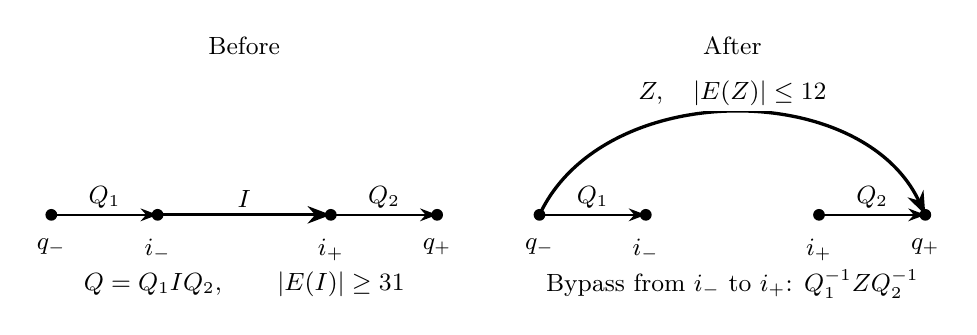
\begin{tikzpicture}[>=Stealth, line width=.7pt,
  every node/.style={font=\small},
  endpoint/.style={circle,fill=black,inner sep=1.5pt},
  pathlabel/.style={fill=white,inner sep=2pt}]
  \begin{scope}
    \node at (2.45,2.15) {Before};
    \coordinate (a) at (0,0);
    \coordinate (b) at (1.35,0);
    \coordinate (c) at (3.55,0);
    \coordinate (d) at (4.90,0);
    \draw[->] (a) -- node[pathlabel,above] {$Q_1$} (b);
    \draw[->,very thick] (b) -- node[pathlabel,above] {$I$} (c);
    \draw[->] (c) -- node[pathlabel,above] {$Q_2$} (d);
    \foreach \q in {a,b,c,d} \node[endpoint] at (\q) {};
    \node[below=5pt] at (a) {$q_-$};
    \node[below=5pt] at (b) {$i_-$};
    \node[below=5pt] at (c) {$i_+$};
    \node[below=5pt] at (d) {$q_+$};
    \node at (2.45,-.88) {$Q=Q_1IQ_2,\qquad |E(I)|\ge31$};
  \end{scope}
  \begin{scope}[xshift=6.2cm]
    \node at (2.45,2.15) {After};
    \coordinate (a) at (0,0);
    \coordinate (b) at (1.35,0);
    \coordinate (c) at (3.55,0);
    \coordinate (d) at (4.90,0);
    \draw[->] (a) -- node[pathlabel,above] {$Q_1$} (b);
    \draw[->] (c) -- node[pathlabel,above] {$Q_2$} (d);
    \draw[->,very thick] (a) to[out=65,in=115]
      node[pathlabel,above] {$Z,\quad |E(Z)|\le12$} (d);
    \foreach \q in {a,b,c,d} \node[endpoint] at (\q) {};
    \node[below=5pt] at (a) {$q_-$};
    \node[below=5pt] at (b) {$i_-$};
    \node[below=5pt] at (c) {$i_+$};
    \node[below=5pt] at (d) {$q_+$};
    \node at (2.45,-.88) {Bypass from $i_-$ to $i_+$: $Q_1^{-1}ZQ_2^{-1}$};
  \end{scope}
\end{tikzpicture}
\caption{The shortening move: add $Z$ between the endpoints of $Q$,
then delete the edges and interior vertices of $I$. The retained paths
$Q_1,Q_2$ and the new path give a bypass with the same value in $D$
as $I$. The drawing is schematic: displayed endpoints may coincide,
and $Q_1,Q_2$ may overlap or be empty. The proof establishes that both
avoid the edges and interior vertices of $I$. Each line denotes a path,
and the rest of the graph is omitted.}
\label{rank:shortening-schematic}
\end{figure}


Attach a new path $Z$ between the endpoints of $Q$ with label $z$,
using new interior vertices and $k=|z|\le12$ new edges.  Then delete
the edges and interior vertices of $I$.  The old endpoints of $I$
are still connected by the path
\[
 Q_1^{-1} Z Q_2^{-1},
\]
which avoids everything deleted.  Thus the new graph is connected.
The inserted path has $k-1$ new interior vertices, and the deleted
segment has $\ell-1$ interior vertices, also when either path has
coincident endpoints.  Hence the changes in the numbers of edges
and vertices are both $k-\ell$, and the graph rank is unchanged.
The basepoint survives, since it is not an interior vertex of $I$.

Equation~\eqref{rank:short-word} gives
\[
 [\operatorname{lab}(Q_1^{-1}ZQ_2^{-1})]_D
   =[\operatorname{lab}(I)]_D.
\]
Every reduced loop at $p$ in the old graph that uses an edge of $I$
must traverse all of $I$, in one direction or the other: its interior
vertices have degree two and do not contain $p$.  Replacing each
such traversal by the displayed bypass, or its inverse, gives a loop
in the new graph with the same value in $D$.  The loop-label map of
the new graph therefore remains surjective.  Its edge count has
decreased by at least $31-12=19$, contradicting minimality of $Y$.
This proves the theorem.
\end{proof}

\begin{corollary}\label{rank:asymptotic}
Suppose that a sequence of length-$100$ row systems satisfies
\eqref{rank:expansion} for a fixed $0<\alpha<1/200$, their sizes
$n$ tend to infinity, and their bad-row counts satisfy $b=o(n)$.
Then their presented groups satisfy
\[
 \operatorname{rk}(D)>\frac{\alpha n}{100}
 \quad\text{for all sufficiently large }n,
 \qquad
 \liminf_{n\to\infty}\frac{\operatorname{rk}(D)}n
 \ge\frac\alpha{100}.
\]
\end{corollary}
\begin{proof}
Eventually $\alpha n\ge1$ and $100b\le\alpha n$, so
Theorem~\ref{rank:main} applies.
\end{proof}

\section{Completing the cost comparison}
\label{conclusion:section}

We now combine the measurable and finite arguments on the same group
and the same Bernoulli action.

\begin{proof}[Proof of Theorem~\ref{intro:main}]
Lemma~\ref{actions:normal-form} shows that $\Gamma$ is finitely
generated and that $J$ is infinite. The actions of
Section~\ref{actions:section} are essentially free and p.m.p., and
conull restriction does not change their costs.

Fix $\alpha$ with the inequalities in the theorem, and set
$\eta=\alpha/100>0$. Proposition~\ref{models:sequence} gives exact
finite right $A$-sets $V_k$ of sizes $n_k\to\infty$, with vanishing
fixed-point fractions for every nonidentity $A$-element, expansion
\eqref{models:expansion}, and $b(V_k)=o(n_k)$. For all sufficiently
large $k$, we have $\alpha n_k\ge1$ and
$100b(V_k)\le\alpha n_k$. The row systems defining $D_{V_k}$ then
satisfy every hypothesis of Theorem~\ref{rank:main}. Hence
\[
 \operatorname{rk}(D_{V_k})>\eta n_k
 \quad\text{for all sufficiently large }k.
\]
By Proposition~\ref{models:transfer},
\[
 \delta_X\ge\limsup_{k\to\infty}
       \frac{\operatorname{rk}(D_{V_k})}{n_k}\ge\eta.
\]
Proposition~\ref{deployment:main} therefore gives
\[
 \operatorname{Cost}(\mathcal R_{\Gamma\curvearrowright X})
 \ge1+\delta_X\ge1+\eta.
\]
For every integer $M>100$, Proposition~\ref{actions:low} gives
\[
 \operatorname{Cost}(\mathcal R_{\Gamma\curvearrowright Y_M})
 \le1+99/M.
\]
The $Y_M$-orbits are infinite, because $\Gamma$ is infinite and its
action is free. Corollary~\ref{compression:cost-one} therefore gives
\[
 1\le\operatorname{Cost}(\mathcal R_{\Gamma\curvearrowright Y_M})
       \le1+99/M,
\]
so these costs tend to one as $M\to\infty$.
An integer $M>\max\{100,99/\eta\}$ exists and satisfies
$1+99/M<1+\eta$. The two costs are therefore strictly different,
which proves the theorem.
\end{proof}

\clearpage
\bibliographystyle{plain}
\bibliography{references}
\end{document}
